\documentclass[border=0pt]{standalone}
\usepackage{lmodern}
\usepackage{tikz}
\usepackage{pgfplots}
\usepgfplotslibrary{groupplots}
\pgfplotsset{compat=1.17}
\definecolor{f07min}{HTML}{000000}
\definecolor{f07sg}{HTML}{0072B2}
\definecolor{f07arpls}{HTML}{D55E00}
\begin{document}
\begin{minipage}{181.86mm}
\centering
% figure: P08-F07; panel: f07-pooled-four-fold-m01-c-random-forest; semantic-sha256: a80ccd58447783b6ff83336d15c300b5297f955760921573638eaca3cc08512e
{\bfseries\fontsize{10}{12}\selectfont P08-F07 / RQ-S05 | Random Forest | M01 individual-spectrum predictions | Pooled sensitivity (S)\par}
\vspace{2mm}
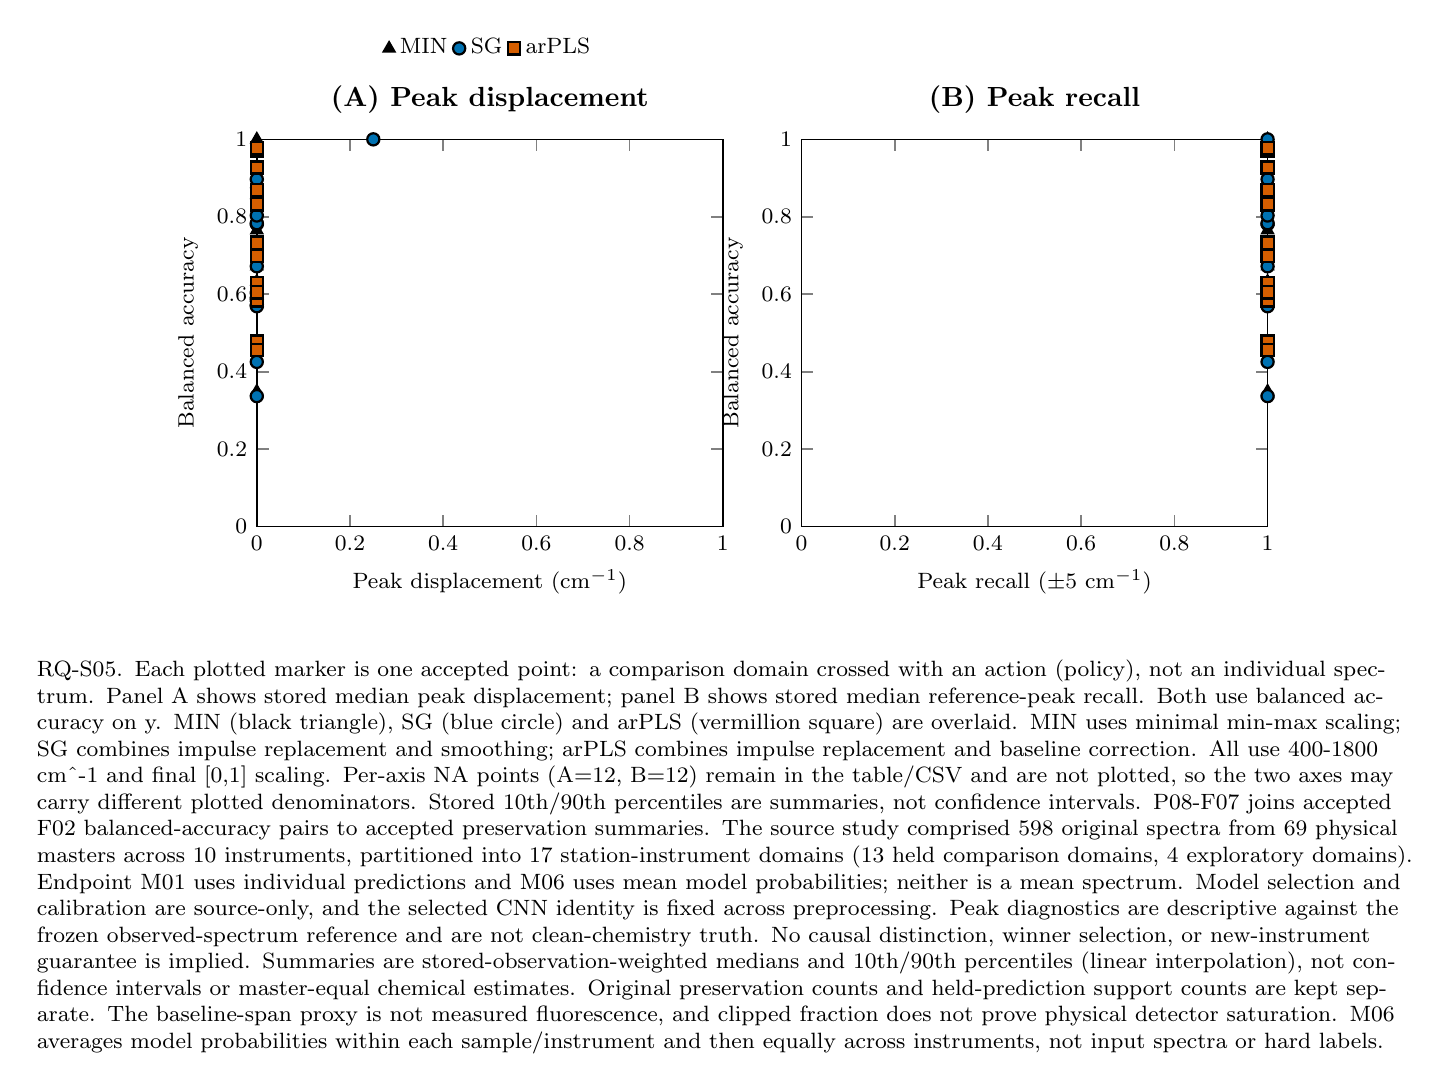
\begin{tikzpicture}
\begin{groupplot}[group style={group size=2 by 1, horizontal sep=10mm, vertical sep=0mm}, width=75mm, height=65mm, clip=false, axis line style={line width=0.6pt}, tick style={line width=0.6pt}, tick label style={font=\fontsize{8}{9.6}\selectfont, black}, label style={font=\fontsize{8}{9.6}\selectfont, black}, title style={font=\bfseries\fontsize{10}{12}\selectfont}, legend style={at={(0.5,1.18)}, anchor=south, draw=none, fill=none, legend columns=3, font=\fontsize{8}{9.6}\selectfont}, ymin=0, ymax=1, ytick={0,0.20000000000000001,0.40000000000000002,0.59999999999999998,0.80000000000000004,1}, yticklabels={0,0.2,0.4,0.6,0.8,1}]
\nextgroupplot[title={(A) Peak displacement}, xlabel={Peak displacement (cm$^{-1}$)}, ylabel={Balanced accuracy}, xmin=0, xmax=1, xtick={0,0.20000000000000001,0.40000000000000002,0.59999999999999998,0.80000000000000004,1}, xticklabels={0,0.2,0.4,0.6,0.8,1}]
\addlegendimage{only marks, mark=triangle*, mark size=2.2pt, mark options={fill=f07min, draw=black, line width=0.8pt}}
\addlegendentry{MIN}
\addlegendimage{only marks, mark=*, mark size=2.2pt, mark options={fill=f07sg, draw=black, line width=0.8pt}}
\addlegendentry{SG}
\addlegendimage{only marks, mark=square*, mark size=2.2pt, mark options={fill=f07arpls, draw=black, line width=0.8pt}}
\addlegendentry{arPLS}
\addplot+[only marks, mark=triangle*, mark size=2.2pt, mark options={fill=f07min, draw=black, line width=0.8pt}] coordinates {(0,0.58111111111111113) (0,0.6010793650793651) (0,0.63296969696969696) (0,0.78712121212121222) (0,0.884848484848485) (0,0.3423655913978495) (0,0.76547619047619053) (0,1) (0,0.34920634920634919) (0,0.59124579124579113) (0,0.85666666666666669) (0,0.67222222222222217) (0,0.61772030651341003)};
\addplot+[only marks, mark=*, mark size=2.2pt, mark options={fill=f07sg, draw=black, line width=0.8pt}] coordinates {(0,0.57277777777777783) (0,0.59064550264550264) (0,0.60339393939393937) (0,0.78106060606060612) (0,0.89696969696969708) (0,0.33703225806451609) (0,0.78339947089947093) (0.25,1) (0,0.42539682539682538) (0,0.56902356902356899) (0,0.80333333333333334) (0,0.67222222222222217) (0,0.58572796934865912)};
\addplot+[only marks, mark=square*, mark size=2.2pt, mark options={fill=f07arpls, draw=black, line width=0.8pt}] coordinates {(0,0.58412698412698405) (0,0.47796825396825399) (0,0.62787878787878793) (0,0.83257575757575764) (0,0.92727272727272736) (0,0.60473655913978486) (0,0.83227513227513228) (0,0.97142857142857153) (0,0.45608465608465609) (0,0.7333333333333335) (0,0.97727272727272729) (0,0.69841269841269837) (0,0.86925287356321834)};
\nextgroupplot[title={(B) Peak recall}, xlabel={Peak recall ($\pm$5 cm$^{-1}$)}, ylabel={Balanced accuracy}, xmin=0, xmax=1, xtick={0,0.20000000000000001,0.40000000000000002,0.59999999999999998,0.80000000000000004,1}, xticklabels={0,0.2,0.4,0.6,0.8,1}]
\addplot+[only marks, mark=triangle*, mark size=2.2pt, mark options={fill=f07min, draw=black, line width=0.8pt}] coordinates {(1,0.58111111111111113) (1,0.6010793650793651) (1,0.63296969696969696) (1,0.78712121212121222) (1,0.884848484848485) (1,0.3423655913978495) (1,0.76547619047619053) (1,1) (1,0.34920634920634919) (1,0.59124579124579113) (1,0.85666666666666669) (1,0.67222222222222217) (1,0.61772030651341003)};
\addplot+[only marks, mark=*, mark size=2.2pt, mark options={fill=f07sg, draw=black, line width=0.8pt}] coordinates {(1,0.57277777777777783) (1,0.59064550264550264) (1,0.60339393939393937) (1,0.78106060606060612) (1,0.89696969696969708) (1,0.33703225806451609) (1,0.78339947089947093) (1,1) (1,0.42539682539682538) (1,0.56902356902356899) (1,0.80333333333333334) (1,0.67222222222222217) (1,0.58572796934865912)};
\addplot+[only marks, mark=square*, mark size=2.2pt, mark options={fill=f07arpls, draw=black, line width=0.8pt}] coordinates {(1,0.58412698412698405) (1,0.47796825396825399) (1,0.62787878787878793) (1,0.83257575757575764) (1,0.92727272727272736) (1,0.60473655913978486) (1,0.83227513227513228) (1,0.97142857142857153) (1,0.45608465608465609) (1,0.7333333333333335) (1,0.97727272727272729) (1,0.69841269841269837) (1,0.86925287356321834)};
\end{groupplot}
\node[anchor=north, yshift=-6mm, text width=175mm, align=left, font=\fontsize{8}{9.6}\selectfont] at (current bounding box.south) {RQ-S05. Each plotted marker is one accepted point: a comparison domain crossed with an action (policy), not an individual spectrum. Panel A shows stored median peak displacement; panel B shows stored median reference-peak recall. Both use balanced accuracy on y. MIN (black triangle), SG (blue circle) and arPLS (vermillion square) are overlaid. MIN uses minimal min-max scaling; SG combines impulse replacement and smoothing; arPLS combines impulse replacement and baseline correction. All use 400-1800 cm\textasciicircum{}-1 and final [0,1] scaling. Per-axis NA points (A=12, B=12) remain in the table/CSV and are not plotted, so the two axes may carry different plotted denominators. Stored 10th/90th percentiles are summaries, not confidence intervals. P08-F07 joins accepted F02 balanced-accuracy pairs to accepted preservation summaries. The source study comprised 598 original spectra from 69 physical masters across 10 instruments, partitioned into 17 station-instrument domains (13 held comparison domains, 4 exploratory domains). Endpoint M01 uses individual predictions and M06 uses mean model probabilities; neither is a mean spectrum. Model selection and calibration are source-only, and the selected CNN identity is fixed across preprocessing. Peak diagnostics are descriptive against the frozen observed-spectrum reference and are not clean-chemistry truth. No causal distinction, winner selection, or new-instrument guarantee is implied. Summaries are stored-observation-weighted medians and 10th/90th percentiles (linear interpolation), not confidence intervals or master-equal chemical estimates. Original preservation counts and held-prediction support counts are kept separate. The baseline-span proxy is not measured fluorescence, and clipped fraction does not prove physical detector saturation. M06 averages model probabilities within each sample/instrument and then equally across instruments, not input spectra or hard labels.};
\end{tikzpicture}
\end{minipage}
\end{document}